Plasma Cash is a plasma construction with much less user data checking \cite{plasma_cash}. It
utilizes Non-Fungible-Tokens (NFTs) to reduce the
user checking requirements to only the NFTs that they own\footnote{Plasma-MVP requires users to be constantly monitoring the plasmachain for fraudulent state transitions, while Plasma Cash requires that users only watch the mainchain about fraudulent exits of coins that they own}. The system's security relies on users fully authenticating a coin's history before accepting it as a payment by utilizing Sparse Merkle Trees, which allow the efficient verification of inclusion and non-inclusion of a transaction in a block, as explained in the next subsection.

\subsection{Sparse Merkle Trees} 

A Merkle Tree is a data structure which allows to succinctly commit to a dataset and prove the inclusion of a part of the committed dataset in $O(log_2(N))$ steps instead of $O(N)$, where $N$ is the number of elements in the dataset, via \textit{Merkle Proofs}. The committed value is called a \textit{Merkle Root}. A Sparse Merkle Tree (SMTs) \cite{sparse_merkle_trees} is an ordered merkle tree, where each element of the dataset is placed at the leaf with the index corresponding the element's index in the dataset. If an element of the dataset was not included in the Merkle Root, its leaf is set to a special default value. 

The inclusion of a transaction spending a coin in a block can be efficiently proven through a Merkle Proof. The same method can be used to prove the non-inclusion of a spend of a coin in a block. A coin can only be spent once per block because only 1 transaction at its slot can ever exist. If a coin was not spent, the leaf is set to the hash of 0. A visual representation of the above is given in Figure \ref{fig:smt}.

\begin{figure}[ht!]
        \centering
        \subfloat[Merkle proof of inclusion for coin A]{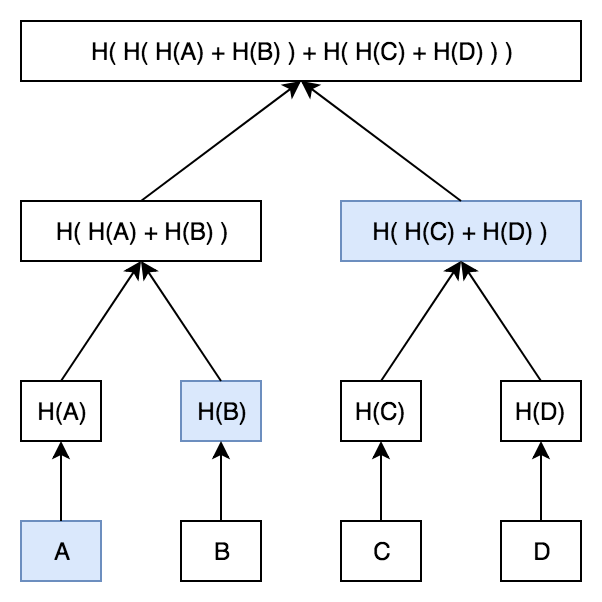
\includegraphics[width=.4\textwidth]{spend}}%
        \qquad
        \subfloat[Merkle proof of non-inclusion for coin C]{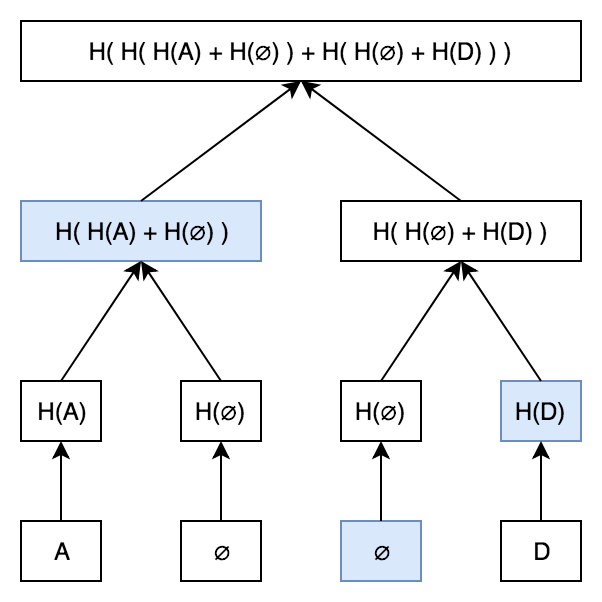
\includegraphics[width=.4\textwidth]{nonspend}}%
    \caption{Merkle Proofs in a Sparse Merkle Tree \cite{smt}}
    \label{fig:smt}
\end{figure}


Further optimizations can be done to the verifier
as suggested in \cite{smt_compact_proofs} by precomputing the default values of
the SMT and by introducing a bitfield in the proof which acts as a
switch between choosing the next 32 bytes during the verification from the
proof or from the SMT's default hashes. A reasonable estimation for a block
containing 2378 transactions results in proof sizes being 320 bytes, compared
to normal proofs which would be 2048 (64 * 32) bytes, for a SMT of size 64.

\subsection{Periodic Merkle Commitments}
All Plasma designs rely on a plasmachain operator that commits the
Merkle Root of each generated block to the mainchain. If a Proof of Stake system is used, publishing a block must be accompanied by a number of validator signatures, exceeding a pre-agreed threshold. 
Whenever a Plasma Block's root is committed to the rootchain, all valid
transactions in that given block can be considered finalized upon availability of the related witness data\footnote{By witness data we refer to the merkle proof of inclusion of that coin in the specified block} for the inclusion of these transactions. Since only the
block root is committed to the mainchain instead of all the included
transactions, plasma can bundle together any number of transactions, the only limit to the number of included transactions being the size of the plasma block. The minimum finality time that
can be achieved is the block time of the rootchain (15 seconds in Ethereum).
Given that every block must be published to the mainchain, the operational costs for this process can become large. Operators can be expected to trade bigger finality time for less maintenance costs by committing block roots less often.


\subsection{Non Fungible Tokens and Depositing a Coin}

When value gets deposited in the plasma smart contract, a unique id and metadata key-value pair gets generated for that token and is saved in the contract's storage. The id is the unique serial number of the coin, and is what makes the deposited coin non-fungible. As a result, depositing 5 ETH two times creates two coins which have their own unique transaction history and are independent from each other. The unique id can also be thought of as a serial number, compared to fiat cash money.

After the coin gets saved in the smart contract, a block containing only the deposit transaction is appended to the plasmachain\footnote{Deposit blocks including only one transaction is an optimization, https://ethresear.ch/t/one-plasma-cash-block-per-deposit-why/2674/}.

% Figure \ref{fig:plasma_cash_deposit} illustrates the process for depositing a
% coin (Ether, ERC20, ERC721, or any other standard) to a Plasma Cash chain. 
% 
% \input{protocols/prot_deposit}
\subsection{Transferring a Coin and Verifying its History}
\label{verify_coin_history}
Each coin in Plasma Cash has its own unique coin history. A coin receiver  must
verify that the coin they are receiving has a valid history in order to accept 
it. A coin with invalid history is counterfeit
and cannot be withdrawn safely. In order to validate a coin's
history, a set of merkle proofs of inclusion
and non-inclusion for the coin since its initial deposit must be sent to the receiver. The receiver can then
proceed to verify that there were no invalid spends of the coin in the coin's
history. This is done by verifying that the proofs of inclusion and non-inclusion are valid
against the plasma block merkle roots that were published to the mainchain.

This imposes a heavy storage and bandwith burden on senders that 
want to transfer a coin. Specifically, the proofs required to send a coin are 
$O(t * log_{2}(N))$ where $t$ is the number of blocks since a coin's deposit and $N$ is the number
of coins the Plasma Cash chain supports.

In a real world scenario where a buyer wants to buy a product from a vendor the
following is expected to happen, in a non-fraudulent case:
\begin{enumerate}
    \item Buyer broadcasts transaction giving ownership of their coin to the
        seller
    \item Transaction gets included in a block and witness data about its inclusion is made available
    \item Buyer verifies that the transaction was included in the block
    \item Buyer sends the proofs of inclusion and non-inclusion to the vendor.
    \item Vendor verifies the history of the coin along with the correct inclusion of the coin's transaction in the block.
    \item Vendor gives the product to buyer
\end{enumerate}

A more elaborate and general protocol for transferring a coin is provided in
Figure \ref{fig:transfer_coin}.

\begin{figure}
\begin{minipage}{\columnwidth}
\begin{framed}
\centering { \bf Protocol for proving and verifying a coin's history } 
%\small

The prover sends two lists of \texttt{IncludedTx} elements to the Verifier, \texttt{inclTx} and \texttt{exclTx}. The verifier has access to the Merkle Roots from the deployed Plasma Contract on Ethereum via the variable \texttt{root[blockNumber]} as well as all the committed block numbers for the coin, via the variable \texttt{blocks}.

We consider a VerifyMerkleProof(slot, hash, proof, blockNumber) algorithm which is able to verify the merkle proof for a coin at a certain block number.

\begin{algorithmic}[1]
    \State ${inclTx, exclTx} \gets proof$
    \State // Ensure completion of included and excluded transactions' blocks
    \State Assert $inclTx.keys \cup exclTx.keys = blocks$ 
    \State // Ensure separation between blocks in included and excluded transactions
    \State Assert $inclTx.keys \cap exclTx.keys = \emptyset$
    \State $LastBlock \gets DepositBlock$
    \State $LastOwner \gets DepositOwner$

    \State // Check the deposit transaction
    \If{!VerifyMerkleProof(slot, inclTx[DepositBlock].tx.hash, itx[DepositBlock].proof, itx[DepositBlock].blkNumber)}
        \State \Return false
    \EndIf
    \State delete inclTx[DepositBlock]
    \State // Check that included transactions are correct in the included blocks
    \For {itx in inclTx} // Skip the deposit transaction
    \If{!VerifyMerkleProof(slot, itx.tx.hash, itx.proof, itx.blkNumber)}
        \State \Return false
    \EndIf

    \State // Reject double spends
    \If{$LastBlock \neq itx.tx.parentBlock$}
        \State \Return false
    \EndIf

    \State // Accept spends only with valid signatures
    \State $Sender \gets ecrecover(itx.tx.hash, itx.tx.sig)$
    \If{$Sender \neq LastOwner$}
        \State \Return false
    \EndIf

    \State $LastBlock \gets itx.blkNumber$
    \State $LastOwner \gets itx.tx.newOwner$
    \EndFor

    \State // Check that there are no transactions in the excluded blocks
    \For {itx in exclTx} // itx.tx should be empty
        \If{!VerifyMerkleProof(slot, emptyHash, itx.proof, itx.blkNumber)}
            \State \Return false
        \EndIf
    \EndFor
\end{algorithmic}


\end{framed}
\end{minipage}
\caption{Proving and verifying a coin's history in Plasma Cash}
\label{fig:transfer_coin}
\end{figure}


\subsection{Exiting and Withdrawing a Coin} \label{exiting_withdrawing}
As described in Section \ref{ch2:classic_plasma}, exits are the mechanism by
which a coin can be withdrawn from the plasmachain, and allow it to be
transferred back to its owner's account on the mainchain. 

Starting an exit for a coin requires providing the transaction that gave the
exitor ownership of the coin signed by the previous owner in the coin's history, as well
as a direct ancestor of that transaction (the reason the parent transaction must also be provided is explained in Section 4). Merkle proofs of inclusion need to also be provided for both transactions.

\begin{figure}[H]
	\makebox[\linewidth]{
		\scalebox{0.6}{
		\includegraphics[width=\linewidth]{figures/coin_exit.pdf}
		}
		}
	\caption{
        Alice deposits a coin from the mainchain to the plasmachain in Block 1. Alice sends the coin to Bob in Block 2. Bob verifies the inclusion of the coin in Block 2. Block 3 gets submitted, without including the coin. Bob sends the coin to Charlie in Block 4. Charlie has to verify the inclusion of the coin in Block 1 and 2, and the non-inclusion of the coin in Block 3. 
        In order for Charlie to exit the coin received by Bob he has to provide
        the signed transaction from Bob as well as a direct ancestor, in this
        case the transaction from Alice to Bob. Charlie also needs to supply
        merkle proofs of inclusion for both of these transactions at their
        respective blocks. 
	}
    \label{fig:exit_lifetime}
\end{figure}

A coin can be modelled by a state machine. After starting an exit, the coin transitions to the \texttt{EXITING} 
state. After the challenge (or maturity) period passes, 
the coin's exit can be finalized and it can transition to the \texttt{EXITED} 
state, from which it can be withdrawn to a user's wallet, 
as shown in Figure
\ref{fig:exit_state_machine}. Figure \ref{fig:exit_lifetime} illustrates the 
lifetime of an exit from its initialization to its finalization. 
We further discuss challenges in Section \ref{ch:attacks}.
\begin{figure}[H]
	\makebox[\linewidth]{
		\scalebox{0.7}{
		\includegraphics[width=\linewidth]{figures/exit_state_machine.pdf}
		}
		}
	\caption{
        The stages of an exit. After a coin transitions to the \texttt{EXITED}
        state, it can be withdrawn to its owner's wallet.
	}
    \label{fig:exit_state_machine}
\end{figure}


\begin{figure}[H]
	\makebox[\linewidth]{
		\scalebox{0.8}{
		\includegraphics[width=\linewidth]{figures/exit_lifetime.pdf}
		}
		}
	\caption{
		During its lifetime, an exit can be challenged during the maturity period. After its maturity period is over, it can be
        finalized and the exiting coin can be withdrawn.
	}
    \label{fig:exit_lifetime}
\end{figure}
